\documentclass[aspectratio=169, dvipdfmx, 11pt]{beamer}
\usepackage{here, amsmath, latexsym, amssymb, bm, ascmac, mathtools, multicol, tcolorbox, subfig, bookmark}

% Design
\usetheme{Madrid}
% Color theme
\usecolortheme{orchid}
% Font theme
\usefonttheme{professionalfonts}
% In frame
\useinnertheme{circles}
% Out of frame
\useoutertheme{infolines}
% Garbage cancellation of bookmark
\usepackage{atbegshi}
\ifnum 42146=\euc"A4A2
\AtBeginShipoutFirst{\special{pdf:tounicode EUC-UCS2}}
\else
\AtBeginShipoutFirst{\special{pdf:tounicode 90ms-RKSJ-UCS2}}
\fi
% Hide navigation bar
\setbeamertemplate{navigation symbols}{}
% Make the default gothic
\renewcommand{\kanjifamilydefault}{\gtdefault}
% Title color
\setbeamercolor{title}{fg=structure, bg=}
% Frame title color
\setbeamercolor{frametitle}{fg=structure, bg=}
% Display slide number only
% \setbeamertemplate{footline}[frame number]
% Itemize
\setbeamertemplate{itemize item}{\small\raise0.5pt\hbox{$\bullet$}}
\setbeamertemplate{itemize subitem}{\tiny\raise1.5pt\hbox{$\blacktriangleright$}}
\setbeamertemplate{itemize subsubitem}{\tiny\raise1.5pt\hbox{$\bigstar$}}
% Color
\newcommand{\red}[1]{\textcolor{red}{#1}}
\newcommand{\green}[1]{\textcolor{green!40!black}{#1}}
\newcommand{\blue}[1]{\textcolor{blue!80!black}{#1}}

\title{論文紹介}
\subtitle{Mask R-CNN}
\author{松永 葵}
\institute{谷口研究室 B4}
\date{2019/04/17}

\begin{document}
\maketitle

\begin{frame}{目次}
    \tableofcontents
\end{frame}

\section{はじめに}
\begin{frame}{目次}
    \tableofcontents[currentsection]
\end{frame}

\begin{frame}{物体検出について}
	\begin{itemize}
    	\item 物体検出
        \begin{itemize}
        	\item 物体を矩形領域で抽出 \\
        \end{itemize}
        \item セマンティックセグメンテーション \\
        \begin{itemize}
        	\item ピクセルひとつひとつにラベルを割り当てる \\
            \item ただし、同じラベルの物体が重なっていると、物体同士の境界がわからない \\
        \end{itemize}
        \item インスタンスセグメンテーション \\
        \begin{itemize}
        	\item 物体検出 + セマンティックセグメンテーション \\
			\item それぞれの物体を区別しつつ、物体がある領域をピクセル単位で分類
        \end{itemize}
    \end{itemize}
\end{frame}


\section{概要}
\begin{frame}{目次}
    \tableofcontents[currentsection]
\end{frame}

\begin{frame}{Mask R-CNNとは}
    \begin{figure}[htb]
		\centering
		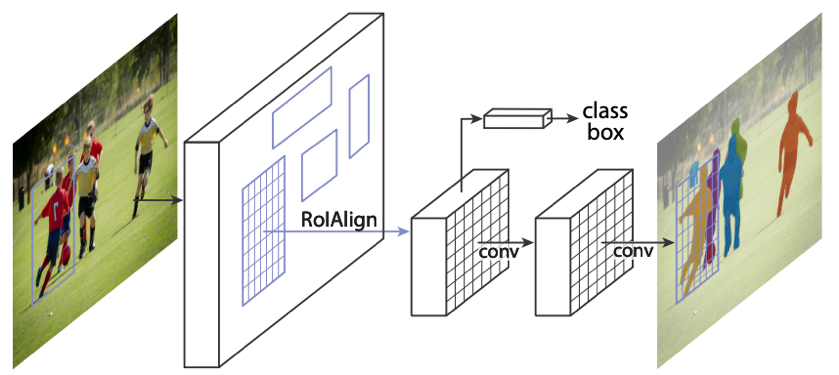
\includegraphics[width=10cm]{./figures/framework.png}
        \caption{The Mask R-CNN framework for instance segmentation.}
    \end{figure}
\end{frame}

\begin{frame}{Mask R-CNNとは}
    \begin{figure}[htb]
		\centering
		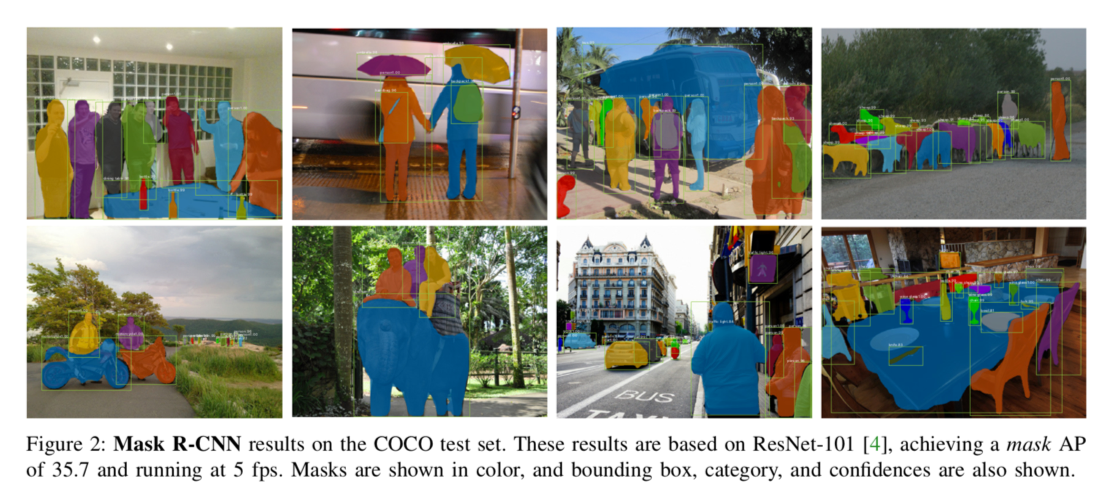
\includegraphics[width=10cm]{./figures/resluts_coco.png}
        \caption{Mask R-CNN results on the COCO test set.}
    \end{figure}
\end{frame}


\begin{frame}{従来手法との違い}
	\begin{itemize}
    	\item セグメンテーション優先戦略 (従来) \\
        \begin{itemize}
        	\item セマンティックセグメンテーション $\rightarrow$ 物体検出 \\
        	\item ピクセルごとの分類から始めて、同じカテゴリのピクセルをインスタンスにカット \\
        \end{itemize}
        \item インスタンス優先戦略 (Mask R-CNN) \\
        \begin{itemize}
        	\item 物体検出とセマンティックセグメンテーションを分離 \\
        \end{itemize}
    \end{itemize}
\end{frame}



\section{物体検出の歴史}
\begin{frame}{目次}
    \tableofcontents[currentsection]
\end{frame}

\begin{frame}{R-CNN (Regional with CNN features)}
    \begin{enumerate}
    	\item Region Proposal \\
        \begin{itemize}
        	\item Selective Search(物体らしさを見つける既存手法)を用いて、
            画像からRoI(物体候補領域)を探す \\
        \end{itemize}
        \item RoIを全て一定の大きさにリサイズしてCNNにかけてfeaturesを抽出 \\
        \item 抽出したfeaturesを使って複数のSVMによって学習しカテゴリ識別Regressionによってbounding boxを推定 \\
    \end{enumerate}

    \begin{figure}[htbp]
        \centering
		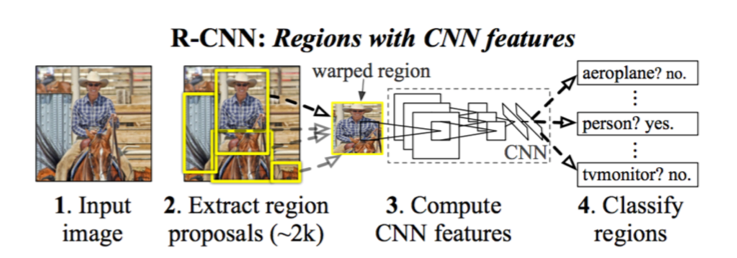
\includegraphics[width=10cm]{./figures/rcnn1.png}
        \caption{R-CNN : Region with CNN features}
    \end{figure}
\end{frame}

\begin{frame}{R-CNN (Regional with CNN features)}
    \begin{itemize}
        \item 物体っぽい領域をたくさん見つけてきて、無理やりリサイズして
        CNNで特徴抽出、SVMでどのクラスか判定 \\
        \item 欠点 \\
        \begin{itemize}
            \item 各項目ごとに別々に学習 \\
            \item 実行時間がめっちゃ遅い \\
        \end{itemize}
    \end{itemize}
    \begin{figure}
        \centering
		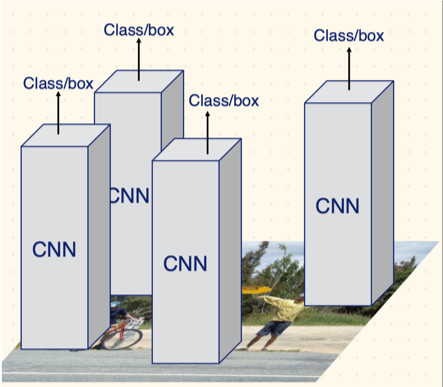
\includegraphics[width=4cm]{./figures/rcnn2.png}
        \caption{R-CNN}
    \end{figure}
\end{frame}


\begin{frame}{Fast R-CNN}
    \begin{itemize}
    	\item RoI pooling layerというシンプルな幅可変poolingを行う \\
    	\item Classification / bounding box regressionを同時に学習させるための、
        multi–task lossによって1回で学習ができるようにする \\
        \item オンラインで教師データを生成する工夫 \\
    \end{itemize}
    \begin{figure}
        \centering
		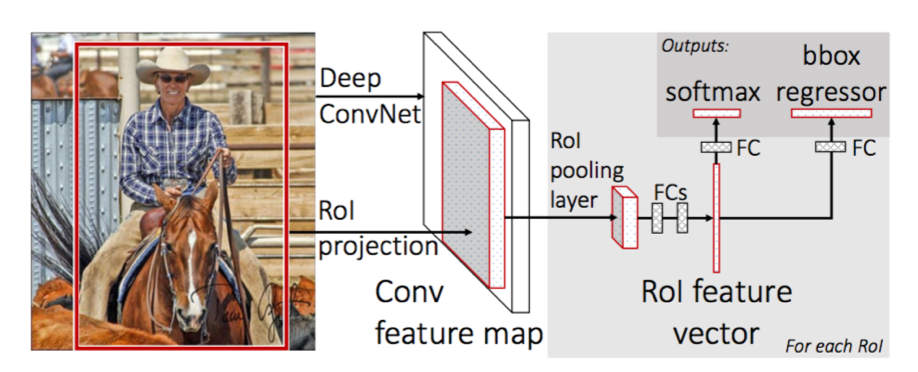
\includegraphics[width=9cm]{./figures/fast_rcnn1.png}
        \caption{Fast R-CNN}
    \end{figure}
\end{frame}

\begin{frame}{Fast R-CNN}
    \begin{itemize}
        \item R-CNNでは、fine-tune/classification/bounding box regressionを
        それぞれ別々に学習する必要があったが、multi - task lossの導入により、Back-Propagationが
        全層に適用できるようになったため、全ての層の学習が可能となった(end to endではない) \\
    \end{itemize}
    \begin{figure}
        \centering
		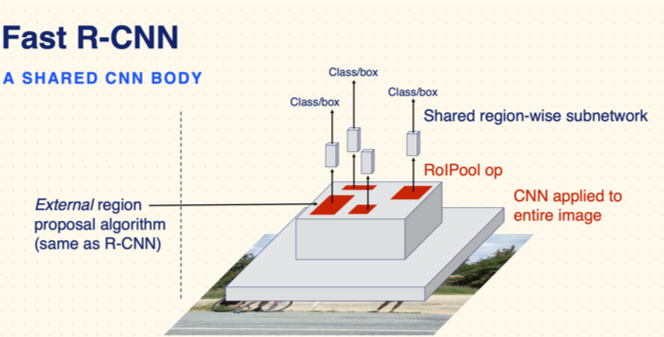
\includegraphics[width=7cm]{./figures/fast_rcnn2.png}
        \caption{Fast R-CNN}
    \end{figure}
\end{frame}


\begin{frame}{Faster R-CNN}
    \begin{itemize}
    	\item Region Proposal Network (RPN)
    	\begin{itemize}
            \item end to end で学習可能 \\
            \item 物体候補領域を推定するネットワーク + RoI Poolingにクラス推定 \\
            \begin{itemize}
                \item 物体かどうかを表すスコア (cls layer) \\
                \item 物体の領域 (reg layer) \\
            \end{itemize}
        \end{itemize}
    \end{itemize}
    \begin{figure}
        \centering
		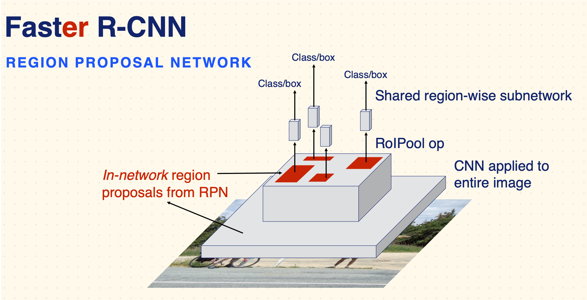
\includegraphics[width=7cm]{./figures/faster_rcnn.png}
        \caption{Faster R-CNN}
    \end{figure}
\end{frame}

\begin{frame}{Faster R-CNN}
    \begin{enumerate}
        \item 画像全体のfeature mapsから予め決められたk個の固定枠(Anchor)
        を用いて特徴を抽出し、RPNの入力とする \\
        \item 各場所について物体候補とすべきか推定 \\
        \item 物体候補として推定された出力枠(reg layer)の範囲を、
        Fast R-CNN同様RoI Poolingし、
        クラスのネットワークの入力とすることで最終的な物体検出を実現 \\
    \end{enumerate}
    \begin{figure}
        \centering
		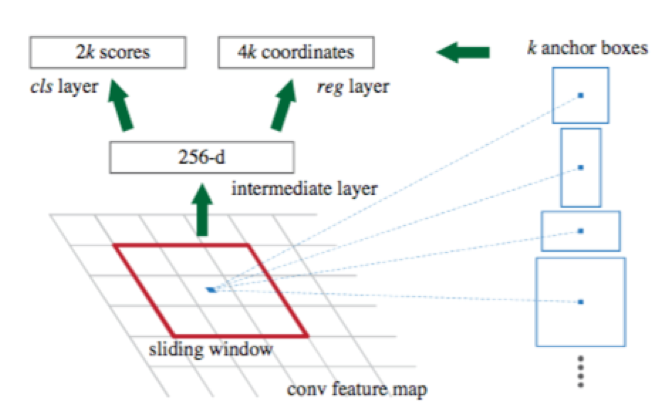
\includegraphics[width=7cm]{./figures/anchor.png}
        \caption{Faster R-CNN}
    \end{figure}
\end{frame}


\section{Mask R-CNN}
\begin{frame}{目次}
    \tableofcontents[currentsection]
\end{frame}

\begin{frame}{Faster R-CNNの拡張}
    \begin{itemize}
        \item 既存のbranchと並行して、mask branchを追加 \\
        \item RoIのセグメンテーションマスクを予測 \\
        \item maskとclassの予測を切り離す \\
        \item RoI Pooling $\rightarrow$ RoI Align \\
    \end{itemize}

    \begin{figure}[htbp]
        \centering
		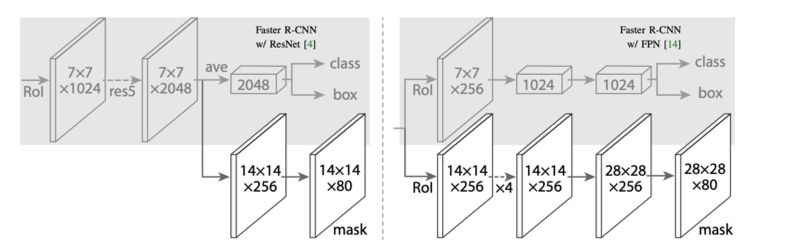
\includegraphics[width=10cm]{./figures/mask1.png}
        \caption{Head Architecture}
    \end{figure}
\end{frame}

\begin{frame}{multi task loss}
    \begin{equation*}
        L = L_{cls} + L_{box} + L_{mask}
    \end{equation*}
    \centering
    (L : RoIごとにサンプリングされたmulti task loss)
    \begin{itemize}
        \item $L_{cls}$ : 分類誤差
        \begin{itemize}
            \item 物体カテゴリ数 + 1クラス分類(+1は背景クラス) \\
            \item 真のクラス$u$に対する事後確率$p^u$の負の対数 \\
            \begin{equation*}
                L_{cls}(p, u) = - \log p^u
            \end{equation*}
        \end{itemize}
        \item $L_{box}$ : 矩形回帰
        \begin{itemize}
            \item 候補領域を真のbounding boxに近づける回帰 \\
            \begin{eqnarray*}
                L_{cls}(v, t) = \sum_{i \in \{x, y, w, h\}} smooth_{L_1}(t_i - v_i) \\
                smooth_{L_1}(x) = \begin{cases}
                    0.5x^2 & if |x| < 1 \\
                    |x| - 0.5 & otherwize
                  \end{cases}
            \end{eqnarray*}
        \end{itemize}
    \end{itemize}
\end{frame}

\begin{frame}{multi task loss}
    \begin{itemize}
        \item $L_{mask}$ : マスク損失
        \begin{itemize}
            \item ピクセルごとのシグモイドを適用し、平均バイナリクロスエントロピー損失として定義
            $L_{mask}$は$k$番目のmaskでのみ定義 \\
            \begin{equation*}
                L_{mask} = - \frac{1}{m^2} \sum_{1 \leq i, j \leq m} [y_{ij} \log {{\hat{y}}^k}_{ij} + (1 - y_{ij}) \log (1 - {{\hat{y}}^k}_{ij})]
            \end{equation*}
            \centering
            (${{\hat{y}}^k}_{ij}$は同じセルに対する$k$番目のmask予測)
        \end{itemize}
        \item[$\rightarrow$] マスクとクラスの予測を分離
    \end{itemize}

    \begin{figure}[htbp]
        \centering
		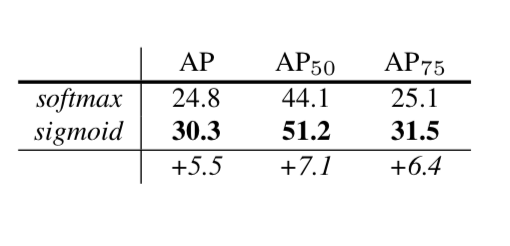
\includegraphics[width=5cm]{./figures/mask2.png}
        \caption{Multinomial vs. Independent Masks (ResNet-50-C4)}
    \end{figure}
\end{frame}

\begin{frame}{(ちなみに)}
    \begin{itemize}
        \item FCNs \\
        \begin{itemize}
            \item ピクセルごとのマルチクラス分類 \\
            \item ソフトマックスと多項クロスエントロピー損失 \\
            \item[$\rightarrow$] セグメンテーションと分類を統合している \\
            \item インスタンスセグメンテーションには向いていない \\
        \end{itemize}
    \end{itemize}
\end{frame}


\begin{frame}{RoI Pooling}
    \begin{itemize}
        \item ピクセル間の空間情報を維持するためのもの \\
        \item ある程度畳み込み処理を行ったfeature mapからRoIを抽出し、
        あらかじめ定義されたサイズにスケーリング \\
    \end{itemize}

    \begin{figure}[htbp]
        \centering
		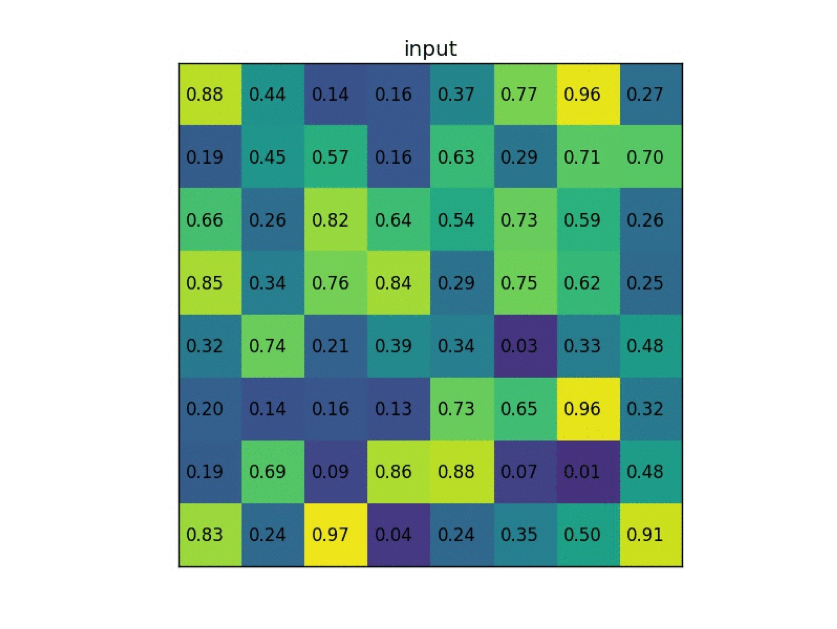
\includegraphics[width=6.5cm]{./figures/roi_pool.png}
        \caption{RoI Pooling}
    \end{figure}
\end{frame}

\begin{frame}{RoI Pooling}
    \begin{itemize}
        \item 元画像のRoIをfeature mapに投影すると、サブピクセルレベルのずれが生じる \\
        \item RoI Poolingでは、このずれを丸め込みながらPoolingを行う \\
    \end{itemize}

    \begin{figure}[htbp]
        \centering
		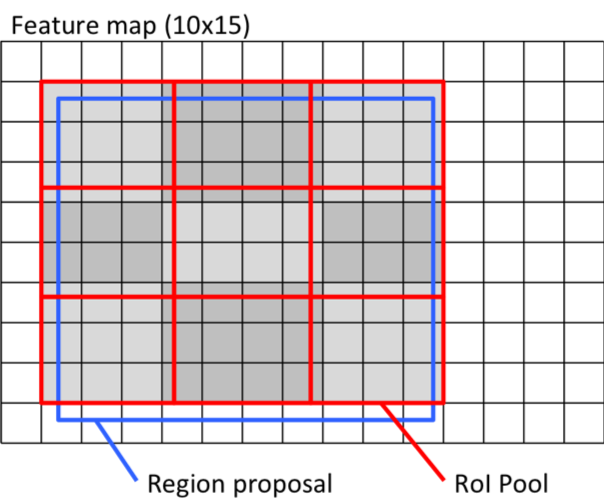
\includegraphics[width=4.5cm]{./figures/feature_map.png}
        \caption{Feature map (10$\times$15)}
    \end{figure}

    \begin{itemize}
        \item[$\rightarrow$] ピクセル精度のmaskを予測するのに多大な悪影響 \\
    \end{itemize}
\end{frame}

\begin{frame}{RoI Align}
    \begin{itemize}
        \item RoI Poolの丸め込みを取り除き、抽出された特徴を入力と正しく位置合わせする \\
    \end{itemize}

    \begin{figure}[htbp]
        \centering
		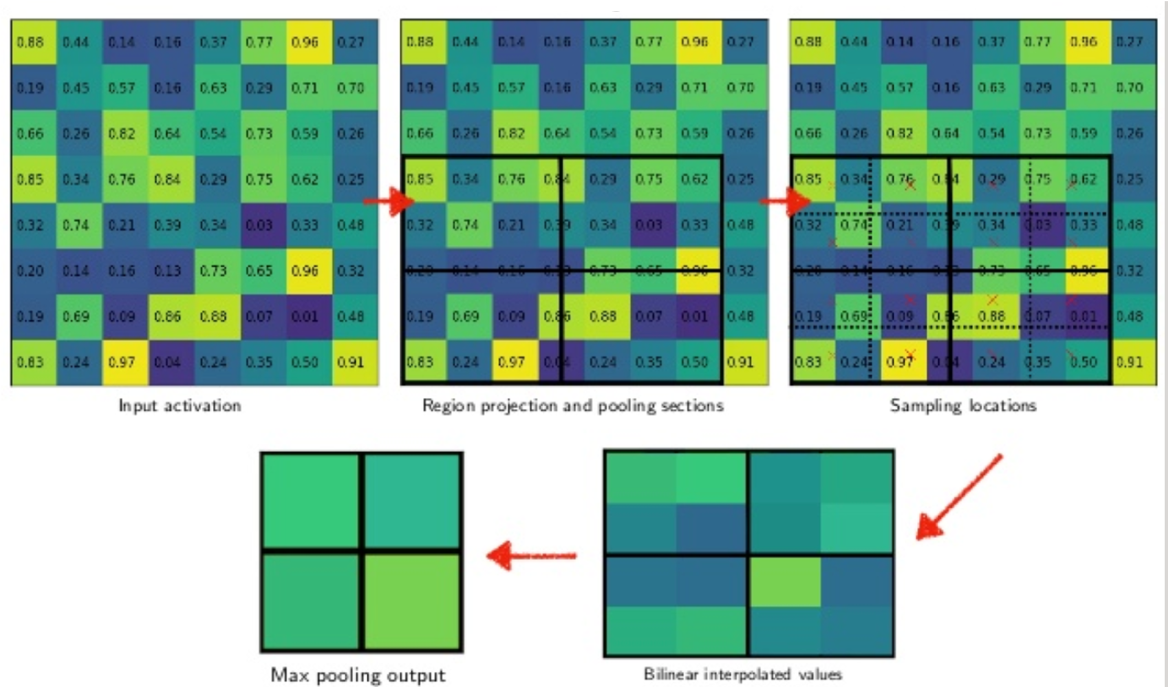
\includegraphics[width=10cm]{./figures/roi_align.png}
        \caption{RoI Align}
    \end{figure}
\end{frame}

\begin{frame}{バイリニア補間}
    \begin{itemize}
        \item 各セル内の4点の近傍4ピクセルからバイリニア補間
        (双線形補間,bilinear interpolation)を用いて
        各点の値を計算する \\
        \item[$\uparrow$] 周囲4画素の画素値の加重平均を計算 \\
    \end{itemize}

    \begin{figure}[htbp]
        \centering
		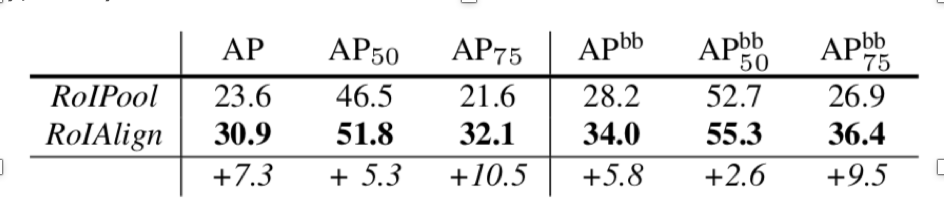
\includegraphics[width=10cm]{./figures/pool_vs_align.png}
        \caption{RoI Align (ResNet-50-C5, stride 32)}
    \end{figure}
\end{frame}


\section{応用分野}
\begin{frame}{目次}
    \tableofcontents[currentsection]
\end{frame}

\begin{frame}{姿勢推定}
    \begin{itemize}
        \item 人間の姿勢推定に容易に拡張が可能
        \begin{itemize}
            \item キーポイントの位置をone-hot maskとしてモデル化 \\
            \item $K$個のキーポイントタイプ(左肩, 右肘など)ごとに一つずつmaskを予測 \\
        \end{itemize}
    \end{itemize}
    \begin{figure}[htbp]
        \centering
		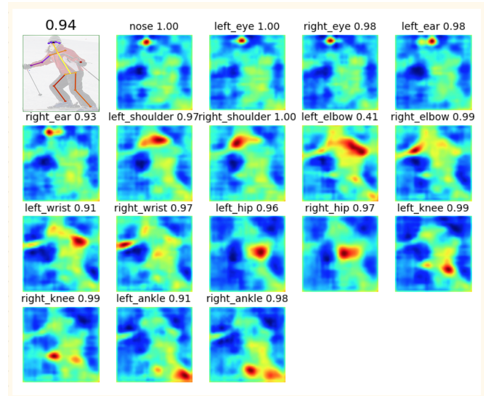
\includegraphics[width=6.5cm]{./figures/one_hot_mask.png}
        \caption{Keypointのone-hot-mask}
    \end{figure}
\end{frame}

\begin{frame}{結果}
    \begin{figure}[htbp]
        \centering
        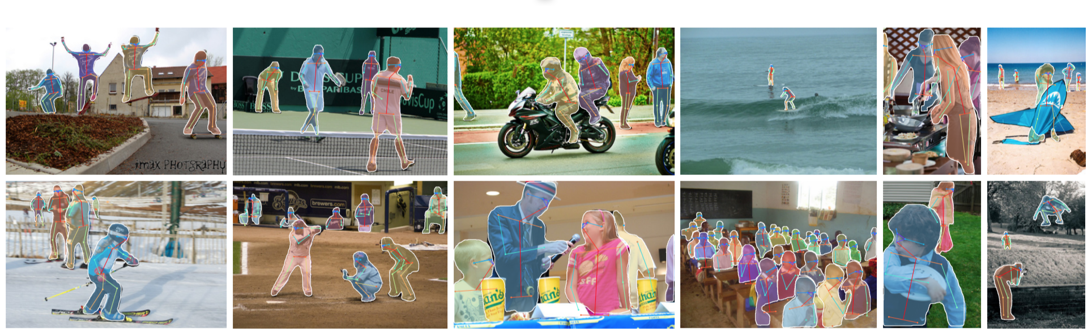
\includegraphics[width=12cm]{./figures/keypoint_coco.png}
        \caption{Keypoint detection resluts on COCO (ResNet-50-FPN)}
    \end{figure}
\end{frame}


\section{結論}
\begin{frame}{目次}
    \tableofcontents[currentsection]
\end{frame}

\begin{frame}{まとめ}
    \begin{itemize}
        \item インスタンスセグメンテーションのためのシンプルで効果的なフレームワーク \\
        \item Faster R-CNNを拡張したもの
        \item 他のタスクへの一般化が容易(論文中では姿勢推定を紹介) \\
    \end{itemize}
\end{frame}

\begin{frame}{感想}
    \begin{itemize}
        \item 今までFaster R-CNNでやっていたものをMask R-CNNでやるというよりは、
        セマンティックセグメンテーションで解決できなかったもの(同じラベルの物体が
        重なった時に境界がわからない)に対して使用するべき? \\
    \end{itemize}
\end{frame}

\begin{frame}[allowframebreaks]{参考文献}
	\begin{thebibliography}{50}
    	\bibitem{bib1} Kaiming He, “Mask R-CNN,” in International Conference on Computer Vision (ICCV), 2017.
    	\bibitem{bib2} R. Girshick, “Fast R-CNN”, in International Conference on Computer Vision(ICCV), 2015.
    	\bibitem{bib3} J. Long, E. Shelhamer, and T. Darrell, “Fully convolutional networks for semantic segmentation”, In Conputer Vision and Pattern Recognition (CVPR), 2016.
    	\bibitem{bib4} http://on-demand.gputechconf.com/gtc/2017/presentation/s7783-ross-girshick-fast-unified-method-object-detection-instance-segmentation-human-pose-estimation.pdf (2019/4/16)
    	\bibitem{bib5} 物体検出についての歴史まとめ \\
        https://qiita.com/mshinoda88/items/9770ee671ea27f2c81a9 \\
        (2019/4/13)
        \bibitem{bib6} 最新の物体検出手法Mask R-CNNのRoI AlignとFast(er) R-CNNのRoI Poolingの違いを正しく理解する \\
        https://qiita.com/yu4u/items/5cbe9db166a5d72f9eb8 \\
        (2019/4/14)
    \end{thebibliography}
\end{frame}


\end{document}
